\documentclass{standalone}
\usepackage{tikz}
\begin{document}
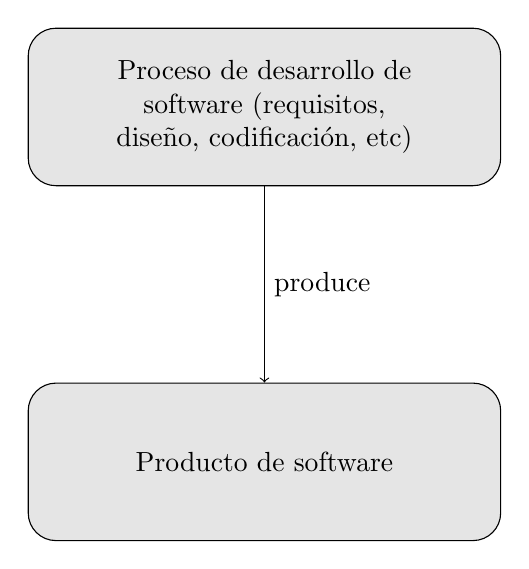
\begin{tikzpicture}
    % Caja superior
    \node[draw, fill=gray!20, rounded corners=10pt, minimum width=6cm, minimum height=2cm, align=center] (proceso) 
        {Proceso de desarrollo de\\ software (requisitos,\\ diseño, codificación, etc)};
        
    % Caja inferior (posicionada manualmente debajo de 'proceso')
    \node[draw, fill=gray!20, rounded corners=10pt, minimum width=6cm, minimum height=2cm, align=center] (producto) 
        at ([yshift=-3.5cm] proceso.south) {Producto de software};
    
    % Flecha con texto
    \draw[->] (proceso.south) -- node[right]{produce} (producto.north);
\end{tikzpicture}
\end{document}
